\documentclass[11pt]{article}
\usepackage{amsmath,amssymb,amsthm}
\usepackage{bm}
\usepackage{algorithm}
\usepackage{algpseudocode}
\usepackage{booktabs}
\usepackage{graphicx}
\usepackage{hyperref}
\usepackage[hmargin=2cm,vmargin=1.8cm]{geometry}
\setlength{\tabcolsep}{4pt}
\graphicspath{{figures/}}

\newcommand{\vpsi}{\bm{\psi}}
\newcommand{\w}{\mathbf{w}}
\newcommand{\R}{\mathbb R}
\DeclareMathOperator*{\argmax}{arg\,max}
\newtheorem{theorem}{Theorem}

\begin{document}
\begin{center}
{\Large Certify-or-Grow and Lazy SF-FSA-VI in stochastic domains: analysis}\\[2pt]
{\small \today}
\end{center}

\noindent This note collects the evidence behind Sections 4--5 of the paper (\texttt{paper/article.tex}): the cost of
building the CCS with \textsc{Certify-or-Grow} (CoG) under noise (\S\ref{sec:ccs}), and Lazy SF-FSA-VI with exact SFs
(\S\ref{sec:mb}) and with learned SFs against the previous algorithm, SF-FSA-VI over the policies of SFOLS
\cite{kuric}, and against Q-learning (\S\ref{sec:mf}). Code, data and commands: \texttt{HANDOFF.md}.

\paragraph{Summary.}
\begin{itemize}\setlength\itemsep{1pt}
\item \textbf{CCS under noise.} The gain of CoG over warm-started SFOLS is smaller than in deterministic domains, and
it needs two implementation details: answering OLS's re-queried extremes with the basis, and continuing the metapolicy
learn (table and visit counts) when the certificate fails. With them, CoG needs $15\%$ fewer steps to converge in
slippery Office ($23\%$ with the model-free certificate) and $8\%$ fewer in the double slit, where it also stops
$2.4\times$ earlier. Without them it was $10\%$ slower in Office. Observations for future work:
\texttt{notes/cog\_stochastic\_observations.md}.
\item \textbf{Lazy SF-FSA-VI with exact SFs} is optimal on all 126 tasks with about 2 added policies per task; keeping
them, a new task is zero-shot (no policy added) in 58--92\% of the cases, 71--97\% in the second half of the sequence.
\item \textbf{Without a model} (oracle certificate on policies and estimates), Lazy SF-FSA-VI brings every windy task
within $0.4\%$ of optimal (zero-shot over the learned extremes: up to $2.1\%$) with about one new policy and 1M steps per
task; once a few policies are stored, 87--97\% of new tasks need none. It needs $2$--$4\times$ fewer samples than
SF-FSA-VI over SFOLS ($21$--$350\times$ after the shared extremes), whose plan even degrades as noisy tables accumulate.
Growing with the metapolicy costs the same per task as Q-learning over all actions ($0.97$--$1.03\times$), but
$2$--$38\%$ less for the new policies that are compositions (certified metapolicy or $\pi^{\mathrm{hyb}}$). Q-learning on the product MDP is $120\times$
more expensive per task in windy, but in Office it is cheaper than learning the extremes (they pay off after 85--155
tasks).
\end{itemize}

% ------------------------------------------------------------------------------------------------------------------
\section{Certify-or-Grow for the CCS in stochastic domains}\label{sec:ccs}

Protocol of the paper's Figure 1 (\texttt{q\_ccs\_stochastic.py}, 10 seeds): SF Q-learning with step $1/(n+1)^{0.7}$,
$\epsilon$-greedy $0.1$, exploring starts, tight optimistic start; a learn stops when its greedy policy is unchanged
for 30 checks of 1000 steps (and every pair has 30 visits) or at the step cap (3M Office, 5M double slit); ``steps to
converge'' is the last check where the greedy value at the start is more than $10^{-3}$ below the optimum (oracle).
Certificate tolerance $10^{-2}$; the model-free version completes the pairs outside $B(s)$ with 100 samples each. CoG
learns its 2nd..$d$-th extreme warm-started, as SFOLS + warm start (\texttt{QBASISWARM=1}). E5 is the first version;
E5b (\texttt{QREUSE=1 QFALLBACK=continue}, the paper's Figure 2) answers OLS's queries at the extremes with the basis
and, after a failed certificate, continues the metapolicy learn over all actions from its table and visit counts (the
entries outside $B(s)$ from GPI over the basis and pool, or from the completion samples).

\begin{table}[h]\centering\small
\caption{Model-free CCS construction under noise: mean $\pm$ std over 10 seeds (Figure
\texttt{q\_ccs\_cost\_stochastic.pdf}). Office: slip $0.05$, $\varepsilon$-CCS with $\varepsilon=0.05$. Double slit:
wind $\pm1$, $\gamma=0.99$, $\varepsilon=10^{-3}$.}\label{tab:ccs}
\begin{tabular}{lcccc}
\toprule
& \multicolumn{2}{c}{Office, slip $0.05$} & \multicolumn{2}{c}{Double slit, wind $\pm1$}\\
& to converge & all steps & to converge & all steps\\
\midrule
SFOLS & $135.7\pm5.6$M & $191.6\pm8.9$M & $13.2\pm1.3$M & $26.0\pm2.0$M\\
SFOLS + warm start & $133.4\pm5.4$M & $193.2\pm9.4$M & $4.24\pm0.66$M & $30.6\pm2.8$M\\
CoG, model certificate (E5) & $147.4\pm12.6$M & $206.5\pm14.5$M & $4.49\pm1.36$M & $21.3\pm2.7$M\\
CoG, model-free certificate (E5) & $120.9\pm10.9$M & $176.6\pm15.4$M & $4.94\pm1.59$M & $22.5\pm3.8$M\\
CoG, model certificate (E5b) & $\mathbf{113.8\pm4.7}$M & $164.9\pm6.8$M & $\mathbf{3.91\pm0.69}$M & $\mathbf{13.0\pm1.4}$M\\
CoG, model-free certificate (E5b) & $\mathbf{102.5\pm4.7}$M & $\mathbf{150.4\pm9.7}$M & $4.15\pm0.69$M & $13.8\pm2.3$M\\
\bottomrule
\end{tabular}
\end{table}

\begin{itemize}\setlength\itemsep{1pt}
\item \textbf{Where E5 lost samples} (Figure~\ref{fig:breakdown}). OLS first queries the extremes, which CoG had
already learned as its basis, and E5 learned each of them again as a metapolicy (Office 8.1M steps to converge, double
slit 6.7M environment steps). A failed certificate paid a wasted metapolicy learn and a full learn from scratch (Office:
17.5 per run, 21.4M + 32.0M). Together these cancelled the gain on the certified queries ($1.00$M per metapolicy
against $1.33$M per warm full learn).
\item \textbf{E5b.} Reusing the basis removes the first overhead ($147.4\to133.6$M). Warm-starting the fallback with
GPI over all tables helps little ($128.3$M); continuing the metapolicy learn makes a fallback cost $0.88$M instead of
$1.83$M and gives $113.8$M. The CCS quality is unchanged (worst $\varepsilon$-gap over 300 weights $0.0052$--$0.0063$,
warm SFOLS $0.0052$--$0.0062$).
\item \textbf{Double slit.} After the 2 extremes every metapolicy is certified and converges at once, so CoG's steps
to converge are those of the extremes (3.9M); warm SFOLS spends another 0.3M. Restricted to $B(s)$ a learn stops after
$1.2$M steps, while every learn over 4 actions runs to the 5M cap (near-tied actions keep flipping), hence 13M against
31M environment steps.
\item \textbf{Office.} Fallbacks remain (16.9 of 98 queries, 97\% in the first half of the queries) and the failed
metapolicy learns are now the main overhead (21.6M). The restriction is mild: $|B(s)|\approx2.9$ of 4 actions with the
extremes and $3.0$ with 26 basis policies, and under noise each entry must still be learned to the noise level.
\end{itemize}

\begin{figure}[h]\centering
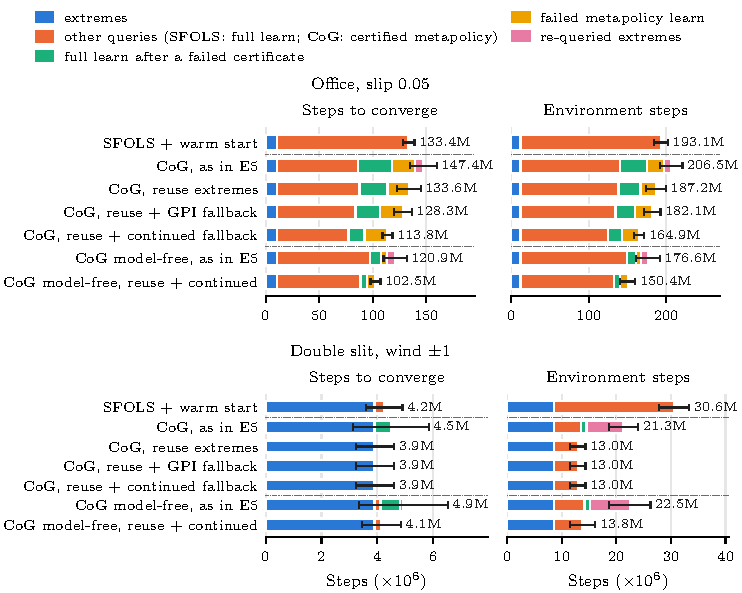
\includegraphics[width=0.9\textwidth]{ccs_cog_breakdown.pdf}
\caption{Where the samples go: mean over 10 seeds of the steps to converge and environment steps by kind of learn,
before (E5) and after (E5b) the two fixes; whisker: std of the total (\texttt{SFOLS/plot\_ccs\_breakdown.py}).}
\label{fig:breakdown}
\end{figure}

% ------------------------------------------------------------------------------------------------------------------
\section{Lazy SF-FSA-VI with the model}\label{sec:mb}

\paragraph{Problem.} SF-FSA-VI \cite{kuric} plans a task automaton over a set of base policies with known SFs. Entering
exit $j$ in automaton state $u$ moves to $\tau(u,j)$: the accepting state $T$, another state $v$, or $u$ itself when the
exit's symbol has no edge from $u$. Exit weights solve
\[
w_j(u)=\begin{cases}1 & \tau(u,j)=T\\ \gamma\,V_{\w(\tau(u,j))}(\varepsilon_j) & \text{otherwise,}\end{cases}
\]
which Kuric et al.\ iterate with $V_\w(\varepsilon_j)=\max_{a,\pi}\vpsi^\pi(\varepsilon_j,a)\cdot\w$ (GPI estimates at
the exits). \emph{Assumption:} the jump into the next automaton state is discounted by $\gamma$ (entering an exit takes a
step), so the iteration is a $\gamma$-contraction even when an exit can be re-entered at once. The iteration is optimal
if the base is a CCS. In stochastic domains the CCS is large (117--572 policies for the $\epsilon$-CCSs below) and an
$\epsilon$-CCS is not exact.

\paragraph{Idea.} The planner only reads values at the weights $\w(u)$ it visits, and these converge. So instead of a
CCS, start from the $d$ extremes and add a policy only at a visited weight where the base is provably not exact.
\emph{Certificate:} the GPI estimate $\hat Q_\w=\max_j Q^{\pi_j}_\w$ is a lower bound with $T\hat Q_\w\ge\hat Q_\w$, so
$T\hat Q_\w=\hat Q_\w$ (one lookahead) implies $\hat Q_\w=Q^*_\w$. \emph{Growth:} the metapolicy over the base first
(composition), then $\pi^{\mathrm{hyb}}$, then improvement \cite{cog}.

\begin{algorithm}[h]
\caption{Lazy SF-FSA-VI}\label{alg:lazy}
\begin{algorithmic}[1]
\Require base $L$ (the $d$ extremes, or the base left by earlier tasks), task automaton
\Repeat
  \State $W\gets$ fixed point of Kuric's iteration over $L$ (warm-started) \Comment{zero-shot; no low-level solve}
  \For{every automaton state $u$}
    \If{$T\hat Q_{\w(u)}=\hat Q_{\w(u)}$} \textbf{continue} \Comment{certified: GPI over $L$ is exact at $\w(u)$}
    \EndIf
    \State $\pi\gets$ metapolicy over $L$ at $\w(u)$ \Comment{composition of stored policies, actions $B(s)$}
    \If{the Bellman gap of $\pi$ is not zero} $\pi\gets\pi^{\mathrm{hyb}}$, then improve until the gap is zero
    \EndIf
    \State $L\gets L\cup\{\pi\}$ (its SFs) \Comment{one small refinement}
  \EndFor
\Until{no automaton state needed a new policy}
\State execute GPI over $L$ at $\w(u)$ in every $u$
\end{algorithmic}
\end{algorithm}

\begin{theorem}
(i) Every $W$ computed is a lower bound on the optimal weights $W^*$. (ii) Algorithm~\ref{alg:lazy} terminates. (iii)
At termination $W=W^*$ and the executed policy is optimal in the product MDP. (iv) In deterministic domains it adds
nothing.
\end{theorem}
\begin{proof}
(i) GPI estimates are lower bounds and the iteration is monotone. (ii) An uncertified $\w(u)$ has no optimal policy in
$L$ (it would make $\hat Q_{\w(u)}=Q^*_{\w(u)}$), so each added policy is new; there are finitely many deterministic
policies. (iii) At the stop every $\w(u)$ is certified, so the GPI estimates at the exits are $V^*_{\w(u)}$: $W=T_LW=T^*W$,
whose unique fixed point is $W^*$; GPI is greedy for $Q^*_{\w(u)}$ in every $u$. (iv) The $d$ extremes give
$\hat Q_\w=Q^*_\w$ for every $\w$ \cite{note}.
\end{proof}

\begin{table}[t]\centering\small
\caption{With the model. Kuric et al.'s plan over the 6 extremes and over the full $\epsilon$-CCS of SFOLS (Office:
$\epsilon=2\cdot10^{-3}$, windy: $10^{-5}$), and the shortest OLS-order prefix of that CCS that makes it optimal
(executed relative regret $\le10^{-9}$); Algorithm~\ref{alg:lazy} from the 6 extremes on every task (fresh) or with the
base carried over the task sequence (stream). Kinds: policies certified as the metapolicy / $\pi^{\mathrm{hyb}}$ /
after policy iteration. Cost in full sweeps per task (SF tables of added policies included); the baseline solves the
product MDP by value iteration from scratch, without SFs. Planning: $|\mathcal U||\mathcal E||\Pi|\times$ iterations of
Kuric's update per task. 33 Office tasks (the 3 of \cite{kuric} and 30 random), 60 windy tasks.}\label{tab:mb}
\resizebox{\textwidth}{!}{%
\begin{tabular}{lccc}
\toprule
& Office, slip $0.1$ & Office, slip $0.3$ & Windy two-stage\\
\midrule
Kuric, 6 extremes: max relative regret & $1.1\cdot10^{-3}$ & $3.2\cdot10^{-3}$ & $1.4\cdot10^{-2}$\\
Kuric, full $\epsilon$-CCS: max relative regret (size) & $3.1\cdot10^{-6}$ (262) & $2.5\cdot10^{-4}$ (572) & 0 (117)\\
CCS prefix that is optimal: median (never optimal) & -- (17 of 33) & 100 (5 of 33) & 11--15 (0)\\
\midrule
Lazy, regret & 0 & 0 & 0\\
fresh: rounds / policies added per task & 2.15 / 1.79 & 2.61 / 2.42 & 2.00 / 2.20\\
stream: policies added per task / final base & 0.67 / 28 & 0.73 / 30 & 0.12 / 13\\
stream: tasks with no policy added (second half) & 58\% (71\%) & 58\% (71\%) & 92\% (97\%)\\
stream: certificate checks / added, per task & 2.8 / 0.67 & 3.0 / 0.73 & 3.1 / 0.12\\
kinds, fresh: metapolicy / $\pi^{\mathrm{hyb}}$ / PI & 10 / 22 / 27 & 31 / 14 / 35 & 24 / 81 / 27\\
kinds, stream: metapolicy / $\pi^{\mathrm{hyb}}$ / PI & 18 / 2 / 2 & 19 / 4 / 1 & 3 / 4 / 0\\
\midrule
cost per task: lazy fresh / lazy stream & 200 / 72 & 558 / 160 & 229 / 24\\
cost per task: product MDP from scratch & 67 & 130 & 282\\
planning per task: lazy stream / Kuric over the $\epsilon$-CCS & $4.7\cdot10^3$ / $4.7\cdot10^4$ &
$9.6\cdot10^3$ / $1.8\cdot10^5$ & $6.0\cdot10^3$ / $5.9\cdot10^4$\\
\bottomrule
\end{tabular}}
\end{table}

\paragraph{Results (Table~\ref{tab:mb}, paper Figure 4).}
\begin{itemize}\setlength\itemsep{2pt}
\item \textbf{Exact with a handful of policies.} Algorithm~\ref{alg:lazy} is optimal on every task in 2--2.6 rounds,
adding about 2 policies per task. With the base carried over, it adds 0.12--0.73 per task and ends with 13--30 policies,
where Kuric's plan needs 11--15 CCS policies per windy task, a median of 100 at slip $0.3$, and is never optimal on half
of the slip-$0.1$ tasks even with all 262. In deterministic Office it adds nothing (Theorem, (iv)).
\item \textbf{It becomes zero-shot.} From the extremes no task passes the exact certificate as it is (a stochastic
optimum always needs some hedging). Keeping the added policies, 58\% of the Office tasks and 92\% of the windy ones are
certified without adding anything, 71\% and 97\% in the second half; a task then costs about 3 certificate checks.
\item \textbf{Refinements are compositions.} With a growing base, 91--100\% of the added policies are the metapolicy
or $\pi^{\mathrm{hyb}}$ over stored policies, with no improvement step over all actions (54--80\% from the extremes; in
windy mostly $\pi^{\mathrm{hyb}}$, the hedging step). Growing by GPI and policy iteration instead adds the same number of
policies, but only 8--71\% are the GPI policy itself.
\item \textbf{Compute.} With the model the lazy plan costs about as much as solving the product MDP in Office (the
metapolicy does not save sweeps over policy iteration), and $12\times$ less in windy once the base has grown. Planning
(Kuric's iteration) is 10--18$\times$ cheaper than over the $\epsilon$-CCS, as $|\Pi|\le30$ instead of 117--572.
\end{itemize}

% ------------------------------------------------------------------------------------------------------------------
\section{Lazy SF-FSA-VI without the model}\label{sec:mf}

\paragraph{Protocol} (\texttt{q\_lazy\_fsa.py}, numba learners of \texttt{mf.py}, 10 seeds, the task sets of
Table~\ref{tab:mb}). Every policy, the $d$ extremes included, is learned by SF Q-learning (step $1/(n+1)^{0.7}$,
$\epsilon$-greedy $0.1$, exploring starts); the model only measures. All methods share the learned extremes.
\begin{itemize}\setlength\itemsep{1pt}
\item \emph{Lazy SF-FSA-VI} (Algorithm~\ref{alg:lazy}). The certificate is replaced by an oracle check (\emph{assumption})
that, at $\w(u)$, the GPI policy and the GPI estimate are within $\delta$ of $V^*_{\w(u)}$ at the start and the exits.
Growth: \emph{metapolicy} (model-free CoG) learns on $B(s)$ until its policy has converged and keeps it if it is
optimal, otherwise continues over all actions; \emph{Q-learning} learns over all actions. Both start at the GPI table.
At most 5 rounds per task.
\item \emph{SF-FSA-VI over SFOLS} \cite{kuric}: OLS corner weights (priority by the improvement bound, $\epsilon=10^{-3}$,
up to 100 queries) from the same extremes, every query learned from the GPI table; after every query, Kuric's plan over
all the learned tables is evaluated on every task.
\item \emph{Q-learning on the product MDP} (Kuric's Flat-Q), from scratch on every task, exploring starts over
$\mathcal U\times\mathcal S$.
\item Learners stop when their greedy policy (and, for SFs, their estimated value) has been within the tolerance of its
optimum for 100 checks of 1000 steps in a row, or at 50M steps (300M for Flat-Q). Tolerances relative to $\max V^*_\w$
at the start and exits: $10^{-3}$ for policies, $10^{-2}$ for estimates; Flat-Q: $10^{-3}V^*$ at the start.
\end{itemize}

\paragraph{What the pilots taught} (\texttt{cluster/sweeps/lazy\_mf\_pilot*.yaml}, 8 tasks, 1 seed).
\begin{itemize}\setlength\itemsep{1pt}
\item \textbf{The certificate must check the estimates.} Checking only the GPI policy at $\w(u)$ certified windy tasks
whose plan had $15\%$ regret: Kuric's iteration reads the \emph{estimates} at the exits, and learned ones can be badly
biased (optimistic start: $4\%$ regret zero-shot; pessimistic: $16\%$). Algorithm~\ref{alg:lazy}'s certificate is a
statement about the estimate, so the oracle version must check it too; with it, every windy task ends within $0.4\%$.
\item \textbf{Pessimistic start.} SF tables start at zero, so learned estimates are biased low and GPI stays an
approximate lower bound, as with exact SFs; an optimistic start ($\Psi=\mathbf e_i$) takes 7--26M steps to unlearn in
windy corridors that cannot reach the exit (0.2--0.4M from zero).
\item \textbf{Estimate tolerance.} Requiring estimates within $10^{-3}$ at every exit is beyond the noise floor of
$1/(n+1)^{0.7}$ steps in Office (extremes capped at 50M); $10^{-2}$ removes the gross biases that break the plan.
\item \textbf{Inherited counts} (warm starts that keep the visit counts of the copied entries, HANDOFF E6) make new
policies $\sim10\times$ slower when the new policy differs from the stored ones (hedging), because the step sizes start
tiny; SFOLS, whose queries are close to stored policies, benefits from them in Office and windy. Each method is
reported with its better setting: Lazy without inherited counts ($4$--$14\times$ cheaper, same regret), SFOLS with
them in windy and Office (cheaper; in windy its plan degrades without them, below) and without them in the double slit.
\end{itemize}

\begin{table}[t]\centering\small
\caption{Without a model: 10 seeds, the task sets of Table~\ref{tab:mb} (double slit: Kuric et al.'s ``blue or red'').
Regrets are relative, at the start state, mean / max over tasks and seeds. ``Kept'': the added policies are carried
over the task sequence. Steps per task exclude the extremes, which every SF method shares. Metapolicy rows: E10d (Algorithm
4's ladder without a model: metapolicy, $\pi^{\mathrm{hyb}}$, all actions; decision after 10 checks).}\label{tab:mf}
\resizebox{\textwidth}{!}{%
\begin{tabular}{lcccc}
\toprule
& Windy & Office, $p=0.1$ & Office, $p=0.3$ & Double slit\\
\midrule
6 (2) learned extremes: steps & 42.6M & 128M & 231M & 33.6M\\
zero-shot over them: regret & $0.90$ / $2.1\%$ & $0.008$ / $0.15\%$ & $0.054$ / $0.33\%$ & $2.1$ / $2.3\%$\\
\midrule
Lazy, metapolicy: new policies, steps per task & 0.85, 1.04M & 0.68, 0.23M & 1.47, 0.81M & 1.00, 2.18M\\
\phantom{Lazy,} regret & $0.17$ / $0.30\%$ & $0.007$ / $0.11\%$ & $0.015$ / $0.15\%$ & $0.031$ / $0.055\%$\\
Lazy, Q-learning: new policies, steps per task & 0.83, 1.04M & 0.68, 0.23M & 1.34, 0.82M & 1.00, 2.26M\\
\phantom{Lazy,} regret & $0.17$ / $0.38\%$ & $0.009$ / $0.11\%$ & $0.011$ / $0.11\%$ & $0.027$ / $0.069\%$\\
kept: tasks with no new policy (second half) & 97\% (100\%) & 91\% (95\%) & 87\% (91\%) & --\\
kept: steps per task, metapolicy / Q-learning & 0.046 / 0.046M & 0.034 / 0.033M & 0.136 / 0.135M & --\\
new policies certified as metapolicy / $\pi^{\mathrm{hyb}}$ & 18 / 14\% & 6 / 20\% & 21 / 28\% & 0 / 0\%\\
\midrule
SF-FSA-VI over SFOLS: steps after the extremes & 61.8M & 384M & 646M & 40.7M\\
\phantom{SF-FSA-VI} regret (queries) & $0.21$ / $0.50\%$ (100) & $0.004$ / $0.11\%$ (100) & $0.021$ / $0.27\%$ (100) &
$0.012$ / $0.045\%$ (8)\\
Q-learning on the product MDP: steps per task & 127M (96\% conv.) & 0.87M & 2.85M & 2.07M\\
\midrule
total steps, SFOLS / Lazy (metapolicy, kept) & $2.3\times$ & $4.0\times$ & $3.7\times$ & $2.1\times$\\
tasks until the SFs beat Q-learning on the product & $<1$ & 153 & 85 & --\\
\bottomrule
\end{tabular}}
\end{table}

\begin{figure}[t]\centering
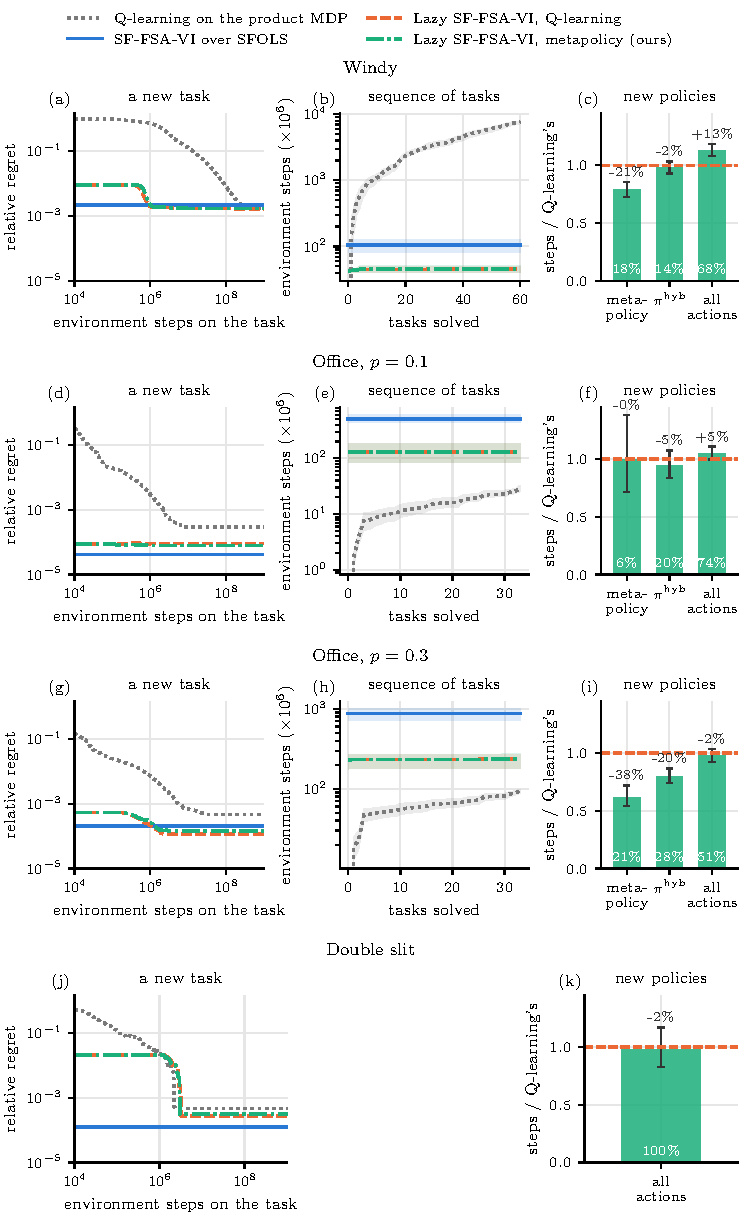
\includegraphics[width=\textwidth]{lazy_mf_all.pdf}
\caption{Without a model, all four domains (paper Figure 5 shows windy and Office $p=0.3$). Left: a new task, relative
regret against the steps spent on it (Lazy from the extremes). Middle: cumulative steps over the task sequence, extremes
included, policies kept. Right: how the metapolicy growth obtained the new policies (share inside the bars) and their
steps relative to Q-learning at the same weight (20 seeds, 95\% interval).}\label{fig:mf}
\end{figure}

\paragraph{Results (Table~\ref{tab:mf}, Figure~\ref{fig:mf}).}
\begin{itemize}\setlength\itemsep{2pt}
\item \textbf{How long a new task takes.} From the extremes: 0.7--1.3 new policies and 0.2--2.3M steps per task (one
policy costs 0.3--2.2M steps, median). With the policies kept: 0.03--0.15M steps per task and 2--3 certificate checks.
\item \textbf{It stays zero-shot.} Kept policies make 87--97\% of the new tasks certified without learning (91--100\%
in the second half of the sequence), as with exact SFs (Table~\ref{tab:mb}). In windy, 80\% of the new policies are the
hedging one at $u_0$, which differs from the nearest stored policy at $\sim220$ of 611 states: it is new behaviour, not a
composition (in Office, a median of 48 of 109 states).
\item \textbf{Metapolicy against Q-learning over all actions} (Figure~\ref{fig:mf}, right). The metapolicy growth
follows Algorithm~\ref{alg:lazy}'s ladder without a model (E10d): learn the metapolicy on $B(s)$ and decide after 10
checks; if it is not certified, complete its table outside $B(s)$ (100 samples per pair, counted) and check
$\pi^{\mathrm{hyb}}$; refine a certified $\pi^{\mathrm{hyb}}$ on $B(s)$ plus its actions (its completed entries count as their
samples), otherwise continue over all actions from the same table. At the same weight, a certified metapolicy needs
$21\%$ (windy) and $38\%$ (Office $p=0.3$) fewer steps than Q-learning and a certified $\pi^{\mathrm{hyb}}$ $2$--$20\%$
fewer, confirmed on 10 held-out seeds; the other new policies pay the metapolicy learning ($+13\%$ in windy, $\pm5\%$
in Office). Compositions are 32\% (windy), 26\% and 49\% (Office) of the new policies, so per task both growths cost
the same ($0.97$--$1.03\times$; seed-to-seed spread $\pm10$--$30\%$). The earlier versions: E10 (decision after 100
checks, $0.98$--$1.4\times$), E10b (10 checks, no $\pi^{\mathrm{hyb}}$, $0.8$--$1.06\times$); trusting the completed entries
in every growth was cheaper on new tasks but made one windy seed's kept library cascade (36 new policies).
Details: \texttt{SFOLS/analyze\_lazy\_growth.py}, \texttt{notes/cog\_stochastic\_observations.md}.
\item \textbf{Against SF-FSA-VI over SFOLS.} SFOLS reaches a similar precision with 40--650M steps on top of the
extremes ($21$--$350\times$ Lazy's) and stores 100 policies (8 in the double slit) instead of 1--7. Without inherited counts its plan
gets \emph{worse} as the set grows (windy: mean regret $\sim10^{-3}$ after 9--17 queries, then 1.3--9.2\% after
62--100): the maximum over many noisy estimates overestimates the exit values. Lazy only adds tables where a task fails
the certificate, so it does not accumulate this bias.
\item \textbf{Against Q-learning on the product MDP.} In windy, $127$M steps per task ($120\times$ Lazy from the
extremes, $\sim3000\times$ with kept policies) and 4\% of the tasks do not converge in 300M. In Office it needs only
0.9--2.9M steps per task, while learning the extremes accurately at every exit costs 128--231M: the SFs pay off after
85--155 tasks. In the double slit (one task) both need about 2M steps per task.
\item \textbf{The cost is the extremes.} As for the CCS, learning SFs accurately is what costs under noise: the shared
extremes are 94--99\% of Lazy's total over the sequence.
\end{itemize}

\paragraph{Limits.} The certificate needs the model or a simulator; with learned SFs it holds only up to their noise.
A sound model-free certificate (confidence bounds from the visit counts) is the main open problem. Termination is
guaranteed with exact SFs, but the number of rounds is not bounded in terms of $d$; without a model it is capped.

{\small
\begin{thebibliography}{9}\setlength\itemsep{0pt}
\bibitem{kuric} D.~Kuric, G.~Infante, V.~G\'omez, A.~Jonsson, H.~van~Hoof. Planning with a learned policy basis to
optimally solve complex tasks. ICAPS 2024.
\bibitem{cog} Certify-or-Grow, \texttt{paper/article.tex}.
\bibitem{note} A small SF basis for SF-FSA-VI, \texttt{notes/gpi\_basis.tex}.
\end{thebibliography}}
\end{document}
